\section{Functional Specification}

This section provides a comprehensive overview of the system's functionality. It includes a use case diagram illustrating the system's interactions and a detailed textual description of each use case.

\subsection{Use Case Diagram}

\begin{figure}[ht]
	\centering
	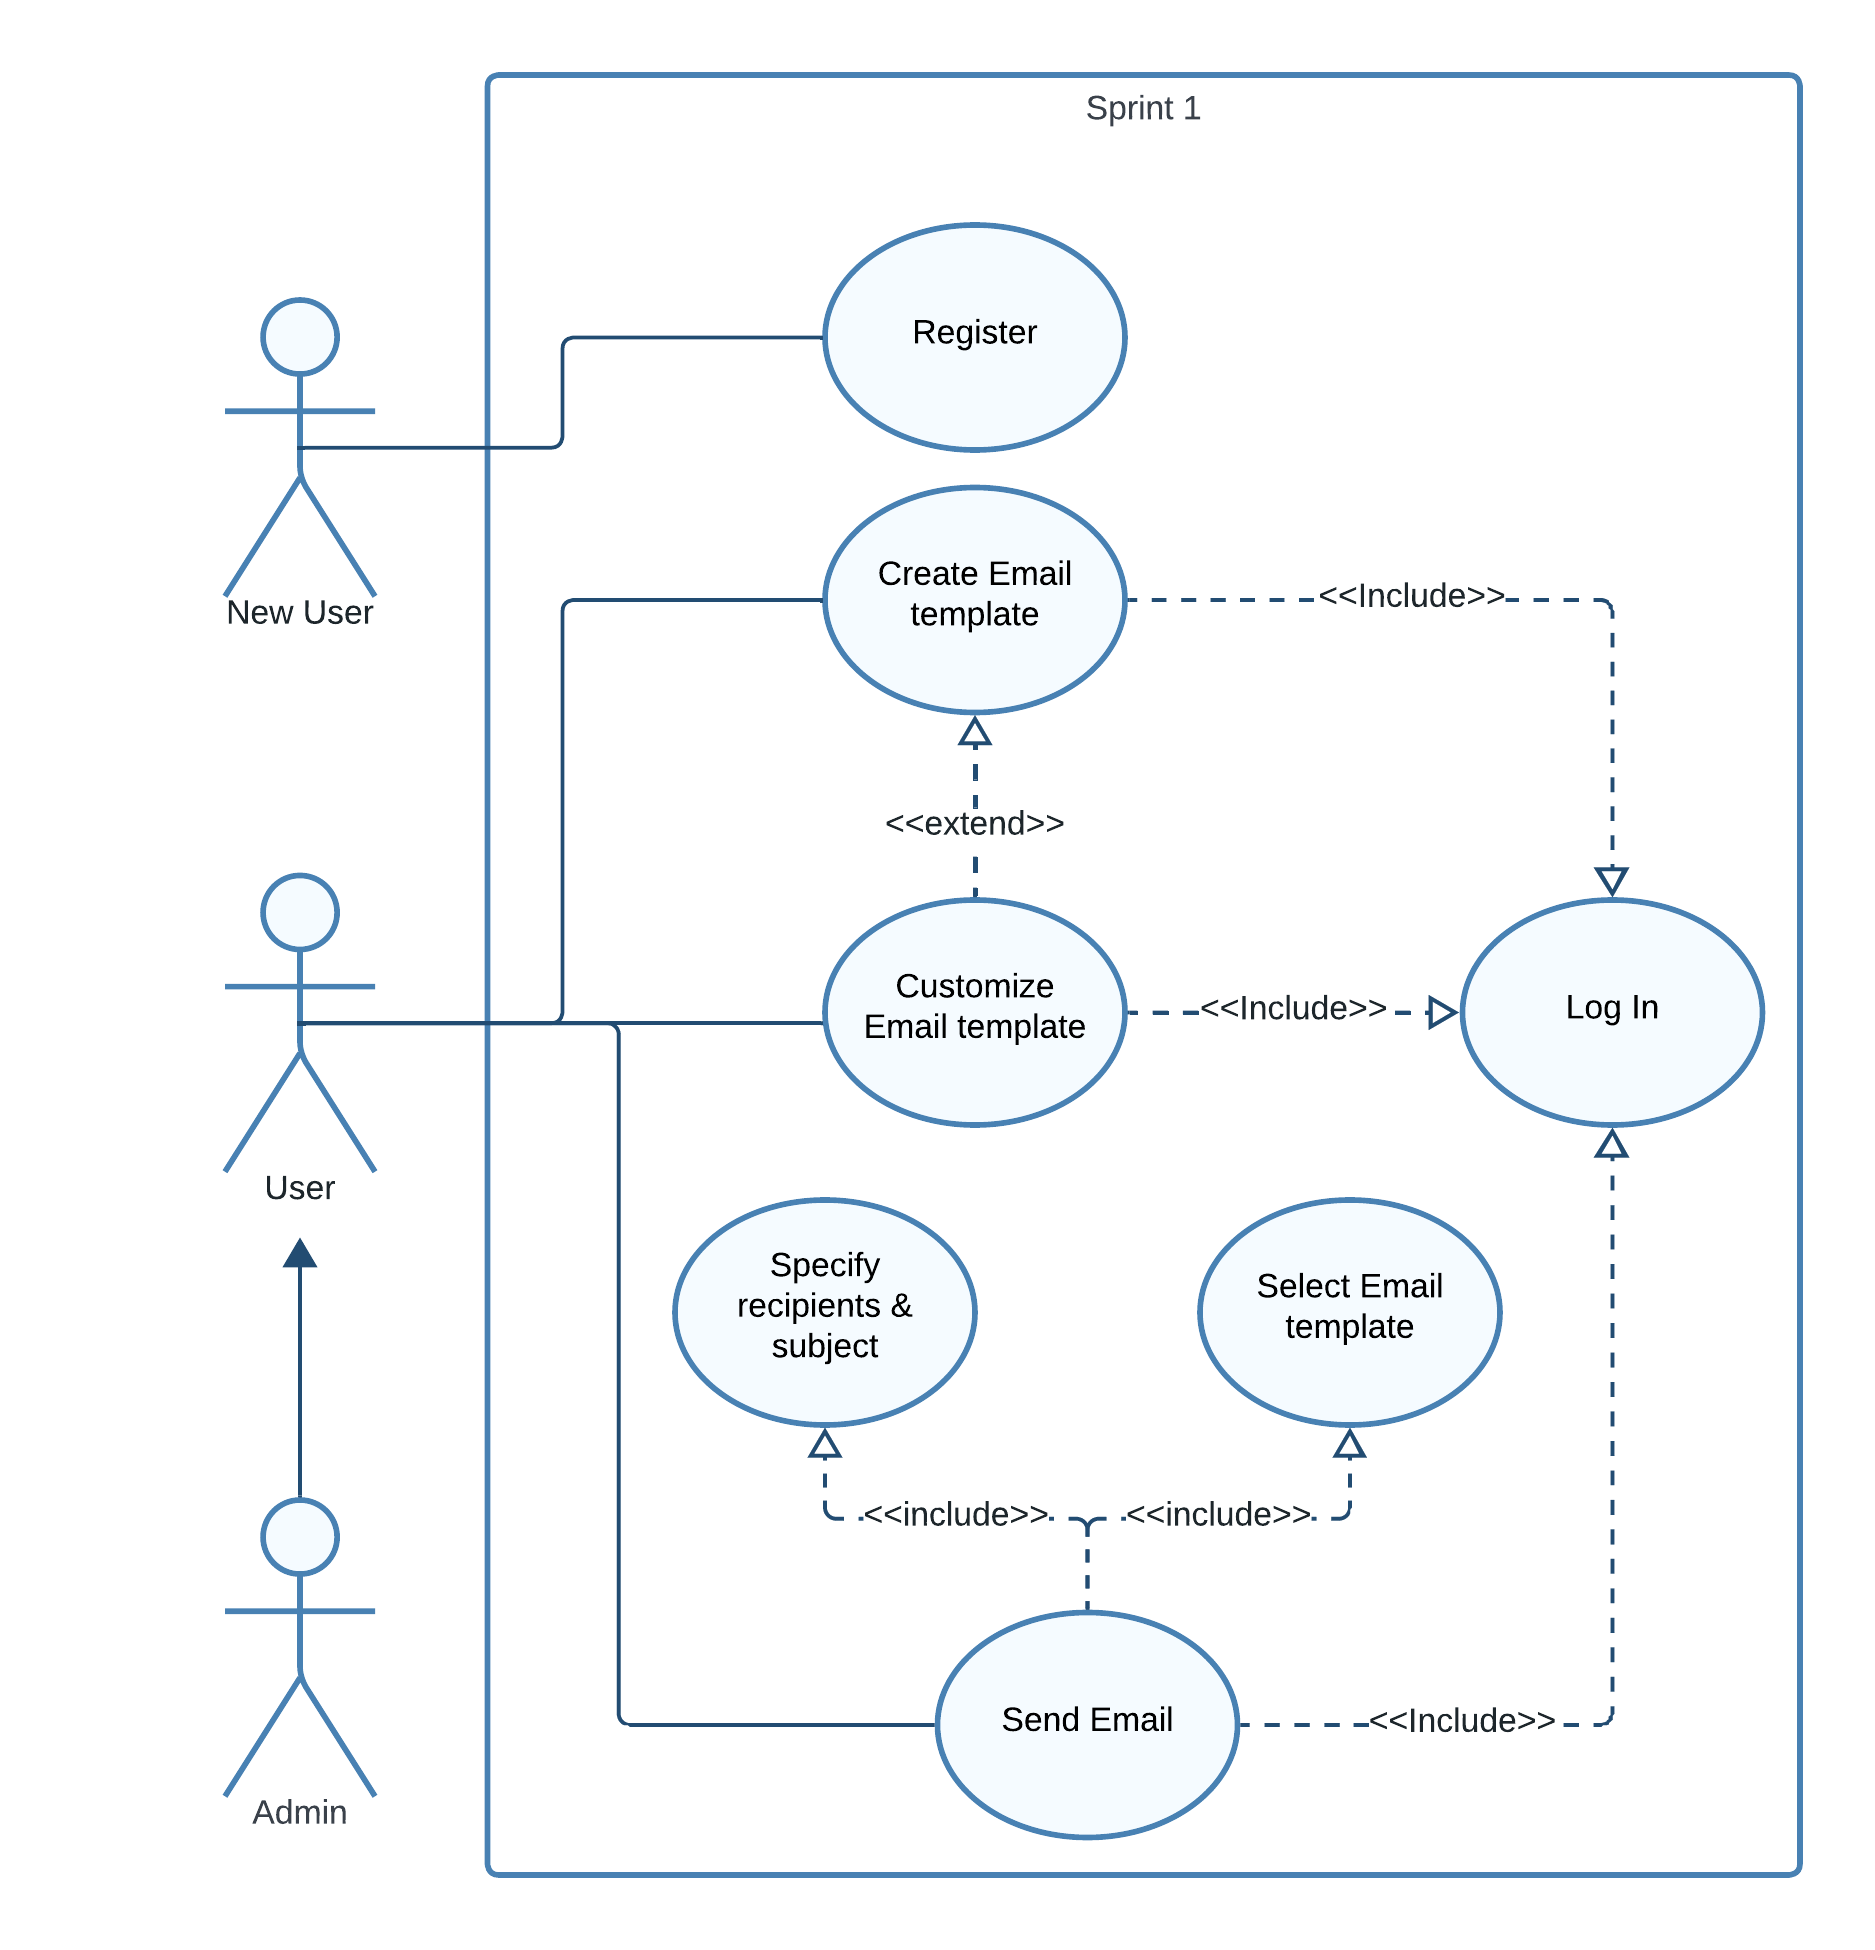
\includegraphics[width=\linewidth]{Images//images/sprint 1 use case diagram.png}
	\caption{Sprint 1 Use Case Diagram}
	\label{fig:Sprint 1 Use Case Diagram}
\end{figure}

\subsection{Textual Description of Use Cases}

The following tables provide a detailed description of each use case. This includes the actor, the system, the goal of the use case, the preconditions, the basic flow, the alternative flows, and the postconditions.

\subsubsection{Use Case 1: Register}

Table 3.2 presents a textual description of a use case: Register.

\begin{table}[ht]
	\centering
	\begin{tabularx}{\textwidth}{|l|X|}
		\hline
		\textbf{Actor}             & New User                                                              \\
		\hline
		\textbf{System}            & Email Marketing Tool                                                  \\
		\hline
		\textbf{Goal}              & To register a new user to the system                                  \\
		\hline
		\textbf{Preconditions}     & The new user has accessed the registration page                       \\
		\hline
		\textbf{Basic Flow}        & 1. The new user enters their details in the registration form         \\
		                           & 2. The system validates the entered details                           \\
		                           & 3. The system creates a new user account                              \\
		\hline
		\textbf{Alternative Flows} & If the entered details are invalid, the system shows an error message \\
		\hline
		\textbf{Postconditions}    & A new user account is created and the new user can log in           \\
		\hline
	\end{tabularx}
	\caption{Use Case 1: Register}
	\label{tab:Use Case 1 Register}
\end{table}

\subsubsection{Use Case 2: Log In}

Table 3.3 presents a textual description of a use case: Log In.

\begin{table}[ht]
	\centering
	\begin{tabularx}{\textwidth}{|l|X|}
		\hline
		\textbf{Actor}             & User, Admin                                                               \\
		\hline
		\textbf{System}            & Email Marketing Tool                                                      \\
		\hline
		\textbf{Goal}              & To authenticate a user to the system                                      \\
		\hline
		\textbf{Preconditions}     & The user has a registered account and has accessed the login page         \\
		\hline
		\textbf{Basic Flow}        & 1. The user enters their login credentials                                \\
		                           & 2. The system validates the entered credentials                           \\
		                           & 3. The system logs the user in                                            \\
		\hline
		\textbf{Alternative Flows} & If the entered credentials are invalid, the system shows an error message \\
		\hline
		\textbf{Postconditions}    & The user is authenticated and logged in to the system                     \\
		\hline
	\end{tabularx}
	\caption{Use Case 2: Authenticate}
	\label{tab:Use Case 2 Authenticate}
\end{table}

\clearpage

\subsubsection{Use Case 3: Create Email Template}

Table 3.4 presents a textual description of a use case: Create Email Template.

\begin{table}[ht]
	\centering
	\begin{tabularx}{\textwidth}{|l|X|}
		\hline
		\textbf{Actor}             & User, Admin                                                  \\
		\hline
		\textbf{System}            & Email Marketing Tool                                         \\
		\hline
		\textbf{Goal}              & To create a new email template                               \\
		\hline
		\textbf{Preconditions}     & The user is authenticated and has accessed the email builder \\
		\hline
		\textbf{Basic Flow}        & 1. The user selects the option to create a new template      \\
		                           & 2. The user designs the template and saves it                \\
		\hline
		\textbf{Alternative Flows} & None                                                         \\
		\hline
		\textbf{Postconditions}    & A new email template is created and saved in the system      \\
		\hline
	\end{tabularx}
	\caption{Use Case 3: Create Email Template}
	\label{tab:Use Case 3 Create Email Template}
\end{table}

\subsubsection{Use Case 4: Customize Email Template}

Table 3.5 presents a textual description of a use case: Customize Email Template.

\begin{table}[ht]
	\centering
	\begin{tabularx}{\textwidth}{|l|X|}
		\hline
		\textbf{Actor}             & User, Admin                                                                                      \\
		\hline
		\textbf{System}            & Email Marketing Tool                                                                             \\
		\hline
		\textbf{Goal}              & To customize an existing email template                                                          \\
		\hline
		\textbf{Preconditions}     & The user is authenticated, has accessed the email builder, and has selected an existing template \\
		\hline
		\textbf{Basic Flow}        & 1. The user makes changes to the selected template                                               \\
		                           & 2. The user saves the changes                                                                    \\
		\hline
		\textbf{Alternative Flows} & None                                                                                             \\
		\hline
		\textbf{Postconditions}    & The selected email template is updated with the new changes                                      \\
		\hline
	\end{tabularx}
	\caption{Use Case 4: Customize Email Template}
	\label{tab:Use Case 4 Customize Email Template}
\end{table}

\clearpage

\subsubsection{Use Case 5: Select Email Template}

Table 3.6 presents a textual description of a use case: Select Email Template.

\begin{table}[ht]
	\centering
	\begin{tabularx}{\textwidth}{|l|X|}
		\hline
		\textbf{Actor}             & User, Admin                                                           \\
		\hline
		\textbf{System}            & Email Marketing Tool                                                  \\
		\hline
		\textbf{Goal}              & To select an email template for sending                               \\
		\hline
		\textbf{Preconditions}     & The user is authenticated and has created at least one email template \\
		\hline
		\textbf{Basic Flow}        & 1. The user navigates to the list of created templates                \\
		                           & 2. The user selects a template for sending                            \\
		\hline
		\textbf{Alternative Flows} & None                                                                  \\
		\hline
		\textbf{Postconditions}    & The user has selected an email template for sending                   \\
		\hline
	\end{tabularx}
	\caption{Use Case 5: Select Email Template}
	\label{tab:Use Case 5 Select Email Template}
\end{table}

\subsubsection{Use Case 6: Specify Recipients and Object}

Table 3.7 presents a textual description of a use case: Specify Recipients and Object.

\begin{table}[ht]
	\centering
	\begin{tabularx}{\textwidth}{|l|X|}
		\hline
		\textbf{Actor}             & User, Admin                                                                \\
		\hline
		\textbf{System}            & Email Marketing Tool                                                       \\
		\hline
		\textbf{Goal}              & To specify the recipients and the subject of the email                                     \\
		\hline
		\textbf{Preconditions}     & The user is authenticated and has selected an email template for sending   \\
		\hline
		\textbf{Basic Flow}        & 1. The user enters the recipient's email address and the Subject                           \\
		                           & 2. The system validates the entered email address                          \\
		\hline
		\textbf{Alternative Flows} & If the entered email address is invalid, the system shows an error message \\
		\hline
		\textbf{Postconditions}    & The recipients and the subject of the email has been specified                              \\
		\hline
	\end{tabularx}
	\caption{Use Case 6: Specify Recipient}
	\label{tab:Use Case 6 Specify Recipient}
\end{table}

\clearpage

\subsubsection{Use Case 7: Send Email}

Table 3.8 presents a textual description of a use case: Send Email.

\begin{table}[ht]
	\centering
	\begin{tabularx}{\textwidth}{|l|X|}
		\hline
		\textbf{Actor}             & User, Admin                                                                                \\
		\hline
		\textbf{System}            & Email Marketing Tool                                                                       \\
		\hline
		\textbf{Goal}              & To send an email                                                                           \\
		\hline
		\textbf{Preconditions}     & The user is authenticated, has selected an email template, and has specified the recipient \\
		\hline
		\textbf{Basic Flow}        & 1. The user clicks the send button                                                         \\
		                           & 2. The system sends the email to the specified recipient                                   \\
		\hline
		\textbf{Alternative Flows} & None                                                                                       \\
		\hline
		\textbf{Postconditions}    & The email has been sent to the specified recipient                                         \\
		\hline
	\end{tabularx}
	\caption{Use Case 7: Send Email}
	\label{tab:Use Case 7 Send Email}
\end{table}
